\documentclass[10pt,a4paper]{article}
\usepackage[utf8]{inputenc}
\usepackage{amsmath}
\usepackage{amsfonts}
\usepackage{amssymb}
\usepackage[pdftex]{graphicx}
\usepackage[colorlinks=true, hidelinks]{hyperref}
\usepackage{listings}
\usepackage[romanian]{babel}
\newcommand{\HRule}{\rule{\linewidth}{0.5mm}}
\lstset{language=VHDL}
\graphicspath{ {img/} }

\begin{document}

\begin{titlepage}
\begin{center}

\textsc{\LARGE Universitatea Tehnica Cluj-Napoca}\\[1.5cm]

\textsc{\Large Facultatea de Automatica si Calculatoare}\\[0.5cm]

% Title
\HRule \\[0.4cm]
{ \huge \bfseries Osciloscop Digital}\\[0.4cm]

\HRule \\[1.5cm]

% Author and supervisor
\begin{minipage}[t]{0.4\textwidth}
\begin{flushleft} \large
\emph{Autori:}\\
% \vspace{3mm}
Alexandru \textsc{Pana}\\
Adrian \textsc{Soucup}\\
gr. 30232
\end{flushleft}
\end{minipage}
\begin{minipage}[t]{0.4\textwidth}
\begin{flushright} \large
\emph{Indrumator:} \\
% \vspace{3mm}
Cristi \textsc{Mocan}
\end{flushright}
\end{minipage}
\vfill

% Bottom of the page
{\large \today}

\end{center}
\end{titlepage}

% TODO
% ---------------------------------------------------------------------------

% Done	Pagina de titlu
% Done	Cuprins (structura documentului anticipata de dumneavoastra)
%  		Introducere (o scurta introducere)
%  		Fundamentare teoretică (pe scurt)
%  		Eventuale Concluzii
% Done 	Bibliografie (numai ce anume credeti dumneavoastra ca va este util)

\tableofcontents

\clearpage

\section{Rezumat}
\paragraph{}
Proiectul de fata isi propune implementarea unui osciloscop digital, folosind o placa de dezvoltare Basys2. Implementarea se va face in limbajul VHDL.

\paragraph{}
In acest document exploram notiounea de osciloscop digital, plecand de la definitie, analizand modul de functionare dar si modul de folosire. Vom analiza componentele necesare implementarii unui osciloscop digital: logica de esantionare, o memorie de esantioane si o logica de iesire. Fiecare componenta este explicata din punct de vedere al functionarii, dupa care se prezinta modul de implementare al acesteia specific pentru placuta de dezvoltare Basys2. Pentru logica de esantionare vom explora utilizarea unui convertor analog digital si logica ce controleaza modul de esantionare. Pentru logica de iesire vom explora portul VGA, ce este acesta, cum functioneaza, si cum este implementat pe placuta Basys2.

In descrierea implementarii proiectului avem in considerare tehnicalitatile specifice placutei de dezvoltare cum ar fi constrangerile, limitarile dar si avantajele acesteia. Vom urmari schema osciloscopului si modul de functionare al acestuia.

In sectiunea de rezultate experimentale se analizeaza functionearea proiectului atat in mediu simulat dar si in mediu real. Se pune in functiune placuta Basys2 si se descriu rezultatele obtinute. Scopul aceste sectiuni este de a demonstra corectitudinea implementarii si functionarii proiectului.

Documentul se incheie cu concluziile autorilor, in care acestia prezinta experienta lor pe parcursul dezvoltarii proiectului, notiunile si lectiile invatate, dar si ganduri despre ce ar putea fi imbunatatit sau adaugat.
\clearpage

\section{Introducere}
% Plasează tema proiectului într-un context mai larg şi furnizează anumite informaţii generale pentru cititor (informaţii mai detaliate vor fi furnizate în secţiunea “Fundamentare teoretică”. 

% Introducerea defineşte de asemenea problema de rezolvat, obiectivele proiectului, descrie pe scurt soluţia propusă şi prezintă conţinutul fiecărei secţiuni următoare din raport.

% • Descrieţi contextul temei proiectului şi tendinţele tehnologice legate de această temă;
% • Definiţi domeniul de studiu, explicaţi terminologia de bază şi descrieţi importanţa
% acestui domeniu;
% • Definiţi clar şi în detaliu problema de rezolvat şi obiectivele principale ale proiectului;
% • Descrieţi pe scurt soluţia propusă şi explicaţi modul în care aceasta este diferită de
% (sau superioară faţă de) alte soluţii existente;

% • În ultimul paragraf al introducerii, prezentaţi ceea ce va conţin fiecare din secţiunile
% următoare ale raportului.

% 2 - 3 pagini. 
% Utilizaţi referinţe la literatura de specialitate sub forma unor numere cuprinse între
% paranteze drepte, ca [1] [5].

\subsection{Osciloscopul Digital}

\paragraph{}
{\bf Osciloscopul} este un aparat electornic de masura ce permite vizualizarea formei unui semnal de voltaj in timp. Osciloscopul este folosit pentru a analiza forma de unda descrisa de un semnal repetitiv. Aceasta vizualizare ofera informatii despre perioada semnalului, amplitudinea acestuia, dar si despre modificari in amplitudine sau perioada. O alta intrebuintare a osciloscoapelor este analiza zgomotelor unui semnal. Fiind aparate de masura ce ofera o reprezentare vizuala detaliata a unui semnal, acestea joaca un rol important in analiza si depanarea circuitelor electrice.

\begin{figure}[h]
\centering
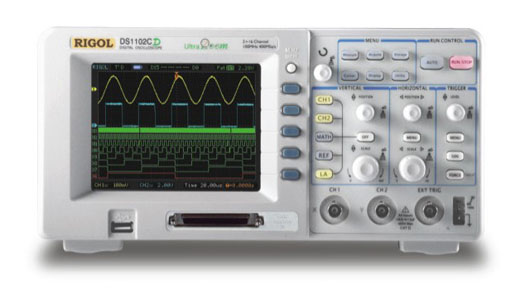
\includegraphics[width=320pt]{digital_oscilloscope}
\caption{Osciloscop Digital}
\label{fig:digital_oscilloscope}
\end{figure}

\paragraph{}
Un osciloscop digital este format din patru componente: un ecran pentru vizualizarea semnalului impreuna cu 3 panori de configuratie ce controleaza dimensiunea amplitudinii semnalului pe monitor, frecventa de esantionare a semnalului, si modul de declansare a esantionarii. Unele osciloscoape digitale ofera posibilitatea masurarii a doua semnale concurent. Aceasta functionalitate este utila daca se urmareste comparatia a doua semnale. De asemenea se pot analiza si semnale digitale daca semnalul analogic de intrare este de asa natura.

\paragraph{}
{\bf Ecranul de vizualizare} este, de cele mai multe ori, un mic monitor CRT integrat in osciloscop. Pe acest monitor se afiseaza semnalul analizat, impreuna cu alte informatii suplimentare cum ar fi o grila de referinta, scala la care este reprezentat semnalul, axele X si Y, sau alti indicatori.

\paragraph{}
{\bf Controlul amplitudinii} este factorul ce determina conversia din valoarea semnalului analogic ( in volti ) in spatiul de afisare al ecranului ( in pixeli ). Folosind acest control putem modifica scala la care este afisat semnalul pe axa Y.

\paragraph{}
{\bf Controlul frecventei de esantionare} ne permite sa modificam frecventa la care osciloscopul citeste semnalul analog. Cu cat frecventa este mai mare, cu atat reconstruirea semnalului pe ecranul de vizualizare este mai fidela. Unele osciloscoape digitale dispun si de un frecventmetru ce le ofera abilitatea de recunoastere a perioadei unui semnal. Pentru ca perioada calculata sa coincida cu cea reala, adica sa nu apara problema de aliasing, frecventa de esantionare trebuie sa fie suficient de mare.

\paragraph{}
{\bf Modul de declansare} a procesului de esantionare determina daca semnalul este esantionat in mod continuu, o singura data sau ca raspuns la un semnal extern. Daca esantionarea se face in mod continuu, imaginea osciloscopului se va schimba constant pentru a reflecta schimbarile semnalului de intrare. Daca esantionarea se face o singura data, monitorul osciloscopului va afisa o imagine statica a semnalului pe o perioada de timp. Daca se alege folosirea unui declansator extern, semnalul va fi esantionat doar la evenimente generate de semnalul declansator.


\subsection{Tema Proiectului}
\paragraph{}
Proiectul de fata isi propune implementarea unui osciloscop digital intr-un limbaj de descriere hardware, pentru a fi sintetizat si rulat pe o placa FPGA.

\paragraph{}
Analizand scopul si modul de functionare a unui osciloscop, se pot observa doua responsabilitati importante ale acestuia:

\begin{description}
	\item[a. Esantionarea semnalului]
		presupune citirea valorii semnalului analogic la intervale regulate, conversia acestora in valori digitale si salvarea acestor esantioane intr-o memorie interna. Vom implementa aceasta responsabilitate intr-un bloc independent. Acest bloc va avea ca intrari semnalul analog de esantionat, impreuna cu valorile de control pentru \emph{frecventa de esantionare} si \emph{modul de declansare}. La iesirile acestui bloc se vor trimite pe rand esantioanele citite.
		
\begin{figure}[h]
	\centering
	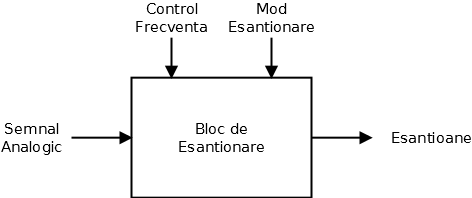
\includegraphics[width=220pt]{bloc_esantionare}
	\caption{Blocul de esantionare}
	\label{fig:bloc_esantionare}
\end{figure}		
		
	\item[a. Afisarea semnalului]		
		presupune reprezentarea esantioanelor prezente in memoria interna pe un ecran. Afisarea poate fi implementata independent de modulul de esantionare, comunicand cu acesta printr-o memorie de esantioane. Blocul de afisare va avea ca intrare memoria de esantionari, iar ca iesire un semnal VGA ce poate fi trimis catre orice monitor.
		
\begin{figure}[h]
	\centering
	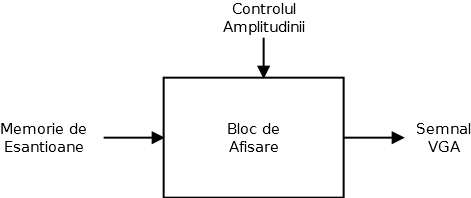
\includegraphics[width=240pt]{bloc_afisare}
	\caption{Blocul de afisare}
	\label{fig:bloc_afisare}
\end{figure}		
\end{description}

\paragraph{}
Cele doua blocuri vor fi implementate separat si vor comunica sincron printr-o memorie de esantioane. Aceasta memorie va contine suficiente esantioane ca sa se poata construi forma de unda pe ecran. Detaliile implementari pot fi gasite in sectiunea urmatoare a documentatiei.


\subsection{Continutul si Structura Documentului}
\paragraph{}
Acest document este impartit in sase sectiuni, fiecare completand si continuand sectiunea anterioara. Aceste sectiuni sunt:

% ---------------------------------------------------------
%	Continutul si Structura Documentului
% ---------------------------------------------------------
\renewcommand{\labelitemi}{$\bullet$}
\begin{description}

	\item[1. Rezumat]
		Aceasta sectiune contine o sinteza scurta a continutului intregului document. Aici sunt prezentate ideile principale din fiecare sectiunie care urmeaza.
		
	\item[2. Introducere] 
		Introducerea are rolul de a plasa problema proiectului in context, de a prezenta scopul proiectului si pozitia acestuia in domeniul studiat. Se analizeaza utilitatea proiectului luand in considerare constragerile platformei pe care este implementat si timpul de dezvoltare al acestuia.
		
	\item[3. Fundamente Teoretice]
		In sectiunea de fundamente teoretice sunt explicate notiunile de baza ale domeniului studiat (analiza semnalelor analogice periodice), implementari similare si o descriere a solutiei propuse. Sunt amintite referintele bibliografice din care s-au documentat autorii.
		
	\item[4. Proiectare si Implementare]
		Aceasta sectiune descrie pe larg structura si implementarea proiectului pe baza notiunilor teoretice prezentate anterior. Este prezentata platforma hardware folosita, impreuna cu deciziile pe care autorii le-au luat la implementarea proiectului.
		
	\item[5. Rezultate Experimetale]
		Aceasta sectiune are rolul de a demonstra corectitudinea implementarii prin exemplificarea functionalitatii. Sunt analizate rezultatele proiectului prin simulare asistata de calculator dar si prin implementarea si rularea sa pe suportul hardware.
		
	\item[6. Concluzii]
		Sectiunea de concluzii cuprinde propriile concluzii ale autorilor, experienta dobandita in urma implementarii proiectului dar si o analiza asupra procesului de implementare si produsul realizat.
		
\end{description}

% ---------------------------------------------------------

\clearpage
\clearpage

\section{Fundamentare teoretica}
\paragraph{}
Osciloscopul este un dispozitiv electronic de testare ce permite 
observarea unor semnale ce variaza constant sub forma unui grafic bidimensional.
Graficul foloseste axa Y pentru a reprezenta valoarea semnalului in functie de timp.

\subsection{Semnalul video VGA}
\paragraph{}
Acesta este semnalul de la iesirea osciloscopului. Folosind un semnal VGA, osciloscopul construit in acest proiect poate fi conectat la orice monitor, si nu necesita unul incorporat. Semnalul VGA este usor de generat, iar majoritatea monitoarelor existente acum au conectori compatibili. In plus, construirea unui monitor integrat care sa afiseze semnalul este in afara scopului acestui proiect. Folosind un monitor extern osciloscopul nostru beneficiaza de o felxibiltate ridicata.

\begin{figure}[h]
\centering
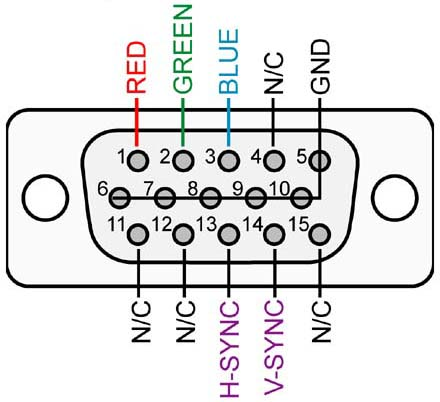
\includegraphics[width=120pt]{vga_pinout}
\caption{Conectorul VGA}
\label{fig:vga_pinout}
\end{figure}

\paragraph{}
Conectorul VGA utilizeaza 5 pini, dintre care 3 pentru culoare ( Rosu, Verde si Albastru ), impreuna cu 2 de sincronizare care reseteaza pozitia fascicolului de electroni pe verticala, respectiv orizontala. Valoarea tensiunii dintre fiecare pin pentru culoare si valoarea tensiunii pinului GND va determina intensitatea canalului respectiv. Pentru a intelege modul de utilizare al pinilor \emph{H-SYNC} si \emph{V-SYNC} trebuie sa intelegem mai intai modul de functionare a fascicolului de electroni in interiorul monitorului.

\begin{figure}[h]
\centering
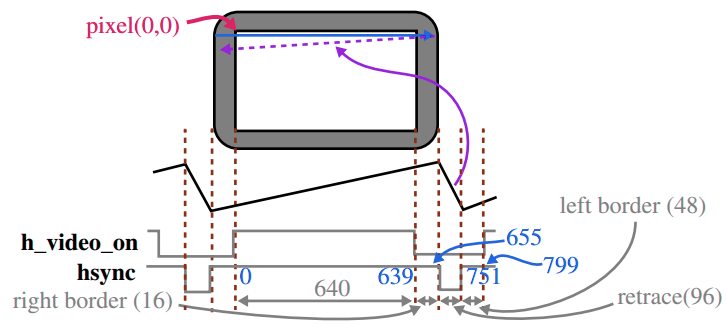
\includegraphics[width=290pt,height=120pt]{vga_timings}
\caption{Timpii de sincronizare VGA}
\label{fig:vga_timings}
\end{figure}

Fascicolul de electroni se misca cu viteza constanta de la stanga monitorului spre dreapta. Se observa totusi ca pozitia de incpeput a acestuia se afla inaintea zonei vizuale. Cand fascicolul de electroni se afla in stanga zonei vizuale, spunem ca se afla la marginea stanga. Definim in mod similar zona marginii drepte. Semnalul {\bf h\_video\_on } din Figura \ref{fig:vga_timings} are valoarea \emph{1} logic cand fascicolul de electroni se afla in zona vizuala, respectiv \emph{0} logic cand acesta se afla fie la marginea stanga, fie la marginea dreapta. Cand fascicolul a ajuns la capatul marginii drepte, se activeaza semnalul \emph{H-SYNC} pentru a incepe resetarea acestuia la marginea dreapta. In concluzie, fascicolul de electorni se poate afla in una din starile urmatoare:

\begin{enumerate}
\item{\bf marginea stanga} atunci cand se afla in stanga zonei vizuale
\item{\bf zona vizuala} cand fascicolul pargurge suprafata monitorului
\item{\bf marginea dreapta} cand fascicolul a depasit suprafata monitorului
\item{\bf curs de intoarcere} cand fascicolul este resetat la inceput
\end{enumerate}

Semnalul \emph{H-SYNC} trebuie sa fie tinut la valoarea \emph{0} in perioada a patra, cand fascicolul este in curs de intoarcere. In functie de rezolutia dorita, si frecventa monitorului, fiecare din aceste stari are o perioada fixa de timp. Semnalul \emph{V-SYNC} are acelasi rol, dar reseteaza fascicolul pe verticala. Deoarece ne vom referi la zonele din afara monitorului atat pe orizontala cat si pe verticala, le vom numi de acum inainte \emph{margine de inceput} si \emph{margine de sfarsit}. Ne vom referi la tabelul urmator pentru informatii despre timpi, considerand o rezolutie de {\tt 640x480}, si o frecventa de {\tt 60Hz}:

\begin{center}
    \begin{tabular}{| l | l | l |}
    \hline
    Stare & Timp Orizontala & Timp Verticala \\ \hline
	margine inceput & 16 & 10  \\ \hline
    zona vizuala & 640 & 480  \\ \hline
    margine sfarsit & 48 & 33 \\ \hline
    intoarcere & 96 & 2 \\ \hline
    total & 800 & 525 \\ 
    \hline
    \end{tabular}
\end{center}

Timpii sunt calculati in impulsuri de clock, iar frecventa clock-ului pentru un monitor de frecventa {\tt 60Hz} este {\tt 25.175MHz}.

\paragraph{}
Valorile semnalelor \emph{Red}, \emph{Green} si \emph{Blue} se schimba la fiecare impuls de clock cand fascicolul de electroni se afla in zona vizuala, pentru fiecare pixel in parte. Cand fascicolul se afla intr-una din marginile exterioare zonei vizuale sau se afla in starea de intoarcere, aceste semnale sunt setate la nivelul \emph{GND}.
\clearpage

\section{Proiectare si implementare}
Osciloscopul va fi format din 3 parti: Logica de intrare, Memoria esantioanelor si logica de iesire.

\begin{figure}[h]
\centering
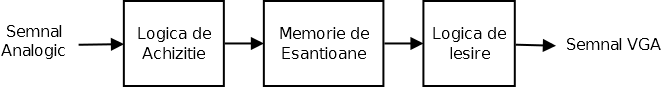
\includegraphics[width=320pt]{block_diagram}
\caption{Schema Block}
\label{fig:block_diagram}
\end{figure}

\paragraph{}
Propunem o implementare in limbaj de descriere hardware a unui osciloscop digital ce poate fi sintetizat pe o placa \textbf{FPGA Basys 2 (Spartan 3E)}. Pentru esantionarea semnalului de intrare vom folosi un convertor analog digital. Vom realiza un protocol de comunicare intre convertor si placuta FPGA astfel incat sa fie usor de schimbat cu alt convertor de exemplu. Frecventa de esantionare a semnalului o vom controla de la switch-uri sau butoane. 
\paragraph{}
Dispunem de o placuta \textbf{CEREBOT II}, placuta care are integrat un  \textbf{convertor AD/10 biti} pe care il putem folosi. Pentru afisarea datelor vom folosi un monitor cu intrare \textbf{VGA}. Placuta Basys 2 dispune de o iesire VGA integrata. Controlul osciloscopului se va face cu ajutorul butoanelor si switch-urilor placutei Basys 2.
\paragraph{}
Ideea de baza a dispozitivului e sa esantioneze un semnal la un interval de timp modificabil si sa salveze pentru fiecare perioada de timp o valoare care reprezinta amplitudinea semnalului de intrare. Dimensiunea intervalului de timp monitorizat este prestabilit sau se poate controla de la switch-uri/butoane. De fiecare data cand intervalul este baleiat vom trimite datele spre controller-ul VGA spre a fi afisate. 
\paragraph{}
Pentru afisarea graficului putem utiliza interpolare spline liniara intre valorile succesive ale amplitudinii semnalului. Cel mai probabil vom avea nevoie de o matrice bidimensionala de pixeli (framebuffer) in care vom desena forma de unda a semnalului de intrare.
\clearpage

\subsection{Blocul de esantionare}

\paragraph{}

Blocul de esantionare este o componenta logica care citeste valorile tensiunii semnalului de intrare la un anumit interval de timp si salveaza in memoria video aceste valori.



\begin{figure}[h]
\centering
\setlength\fboxsep{0pt}
\setlength\fboxrule{0.5pt}
\fbox{
	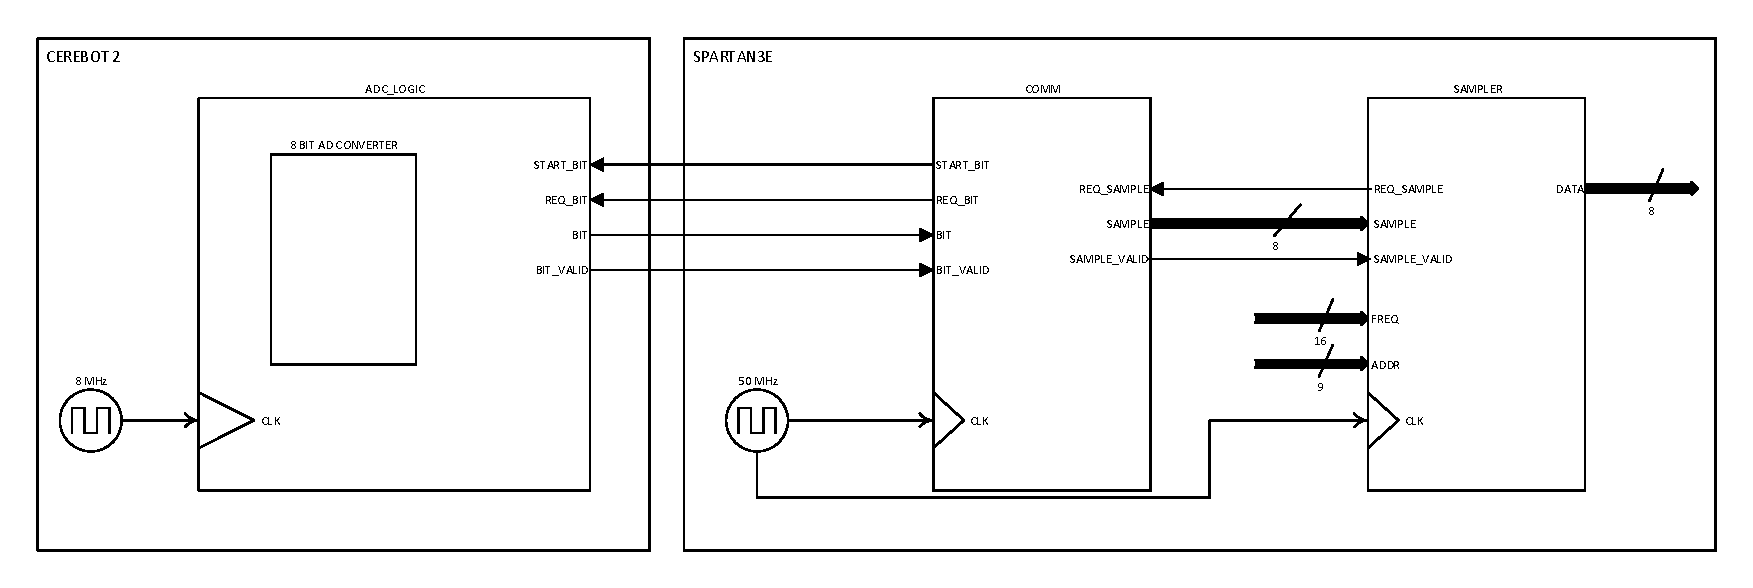
\includegraphics[width=340pt]{oscupdate}
}
\caption{Schema blocului de esantionare cu convertor AD real}
\label{fig:oscupdate}
\end{figure}


\paragraph{}
Acesta este compus din trei subcomponente majore. Componenta ADC, componenta COMM si componenta SAMPLER. Fiecare din aceste componente este un automat de stare.


\paragraph{}
Componenta COMM este responsabila cu transmiterea de informatii dintre convertorul analog digital si componenta de esantionare. Protocolul de comunicare este simplu de inteles si robust. Transmisia bitilor se face in mod serial in pachete de cate 8. In modul IDLE liniile START\_BIT si REQ\_BIT sunt tinute pe zero logic. Cand se doreste transmiterea unui pachet de 8 biti, COMM va trimite un impuls de o lungime fixa (in cazul nostru de 50MHz div 64) pe linia START\_BIT. Dupa o anumita perioada COMM va incepe sa trimita impulsuri pe linia REQ\_BIT de aceiasi lungime cu impulsul de pe START\_BIT. Placuta CEREBOT va detecta aceste impulsuri ca intreruperi externe. Dupa ce s-a trimis un impuls pe REQ\_BIT, COMM va intra intr-o stare de asteptare pana cand linia BIT\_VALID va deveni 1 logic. Este obligatoriu ca aceasta linie sa fie tinuta pe 1 logic pana cand se va transmite un alt impuls pe REQ\_BIT. COMM va citi bitul de pe linia BIT intr-un registru de deplasare, iar mai apoi va trimite din nou o cerere REQ\_BIT pana cand registrul de deplasare este plin.


\begin{figure}[h]
\centering
\setlength\fboxsep{0pt}
\setlength\fboxrule{0.5pt}
\fbox{
	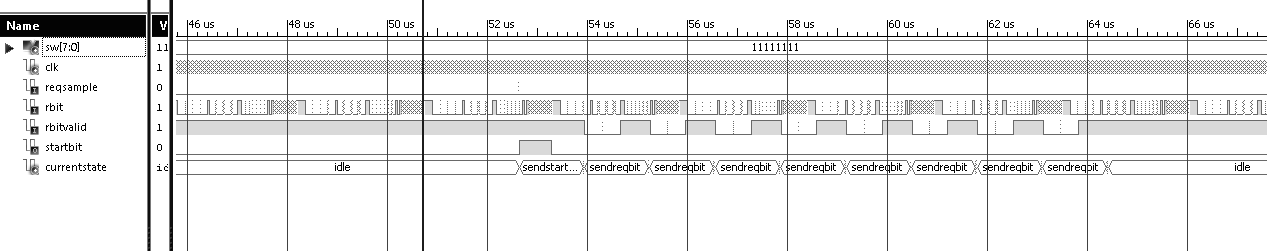
\includegraphics[width=340pt]{waveform-COMM}
}
\caption{Formele de unda pentru COMM}
\label{fig:waveform-COMM}
\end{figure}
\clearpage

\paragraph{}
COMM este un automat de stare. In continuare este prezentata o schema cu tranzitiile intre stari. Starile auxiliare BEGIN* exista deoarece in ele se va intializa un numarator care va avea rolul de a genera impulsuri de o lungime mai mare decat durata tactului de pe placuta FPGA. Avem nevoie de impulsuri mai lungi deoarece placuta CEREBOT2 nu poate detecta intreruperi care sunt mai scurte decat durata clock-ului propriu (8 MHz).

\begin{figure}[h]
\centering
\setlength\fboxsep{0pt}
\setlength\fboxrule{0.5pt}
\fbox{
	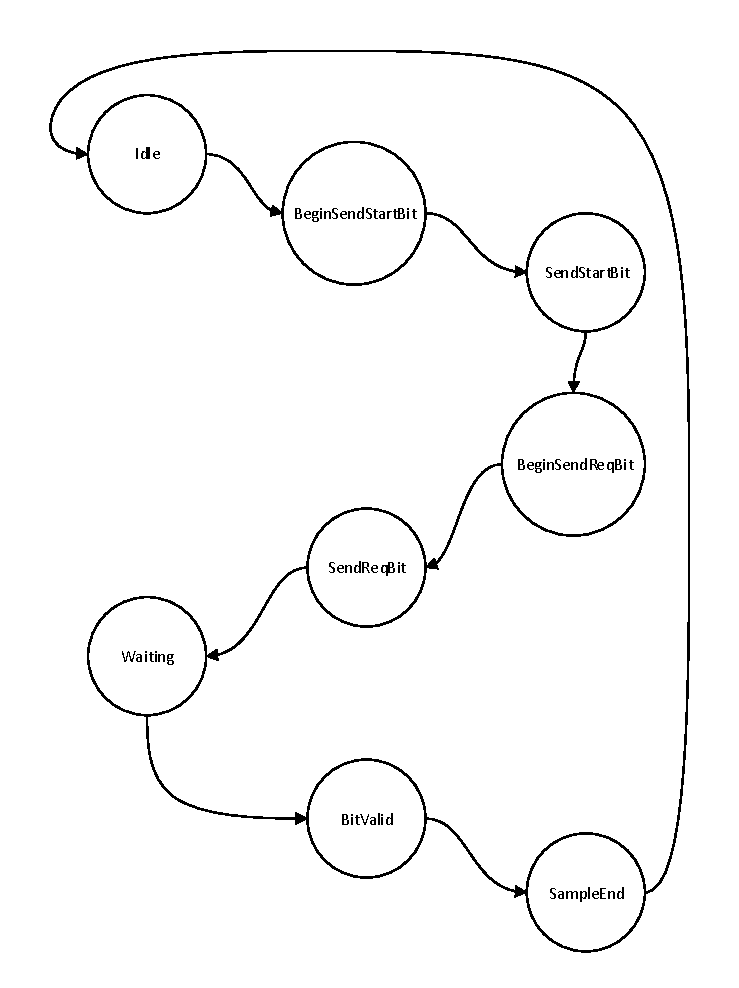
\includegraphics[width=300pt]{COMM-automata}
}
\caption{Diagrama cu tranzitii de stare}
\label{fig:COMM-automata}
\end{figure}
\clearpage


\paragraph{}
Componenta SAMPLER are rolul de declansa conversia analog digitala cu ajutorul bitului REQ\_SAMPLE si a salva valoarea din magistrala SAMPLE cand bitul SAMPLE\_VALID devine 1 intr-o locatie din memoria interna. Memoria video are dimensiunea de 512 x 8 si in ea se vor regasi toate esantioanele capturate. 

\paragraph{}
Frecventa de esantionare este controlata cu variabila FREQ. Aceasta este conectata la SWITCH-urile placutei FPGA si reprezinta numarul de CLK-uri de durata 20ns pe care unitatea sa le astepte intre doua esantioane consecutive.
\(\nu = \frac{1}{ConversionTime + 20ns * FREQ}\)


\paragraph{}
In interiorul componentei se foloseste un registru in care se afla valoarea curenta a adresei de scriere a memoriei. Dupa fiecare esantion capturat valoarea din registru se incrementeaza cu 1, astfel urmatorul sample va fi salvat in continuare in memorie. Exista doua moduri de functionare a osciloscopului: Timp Real si Captura. In modul Timp Real memoria este baleiata si actualizata in mod continuu, in timp ce in modul Captura memoria este actualizata doar atunci cand se detecteaza o schimbare pe portul FREQ.


\paragraph{}
\textbf{Exemplu de functionare}

\begin{figure}[h]
\centering
\setlength\fboxsep{0pt}
\setlength\fboxrule{0.5pt}
\fbox{
	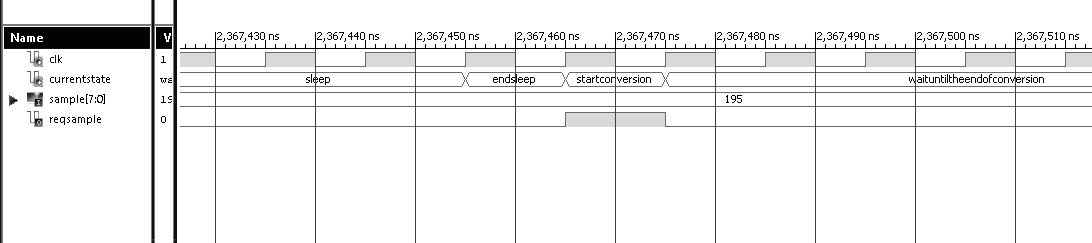
\includegraphics[width=340pt]{waveform-SAMPLER1}
}
\label{fig:waveform-SAMPLER1}
\end{figure}


\begin{figure}[h]
\centering
\setlength\fboxsep{0pt}
\setlength\fboxrule{0.5pt}
\fbox{
	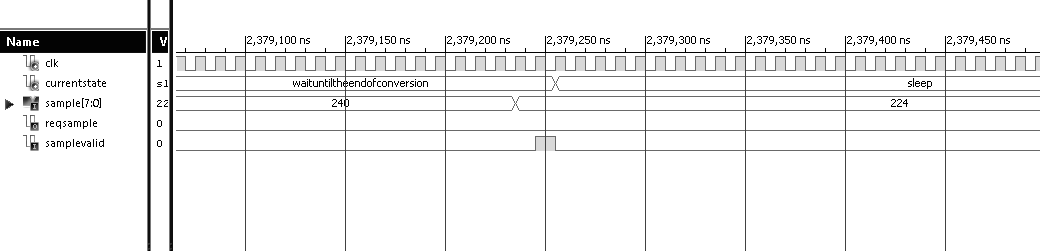
\includegraphics[width=340pt]{waveform-SAMPLER2}
}
\label{fig:waveform-SAMPLER2}
\end{figure}

\begin{figure}[h]
\centering
\setlength\fboxsep{0pt}
\setlength\fboxrule{0.5pt}
\fbox{
	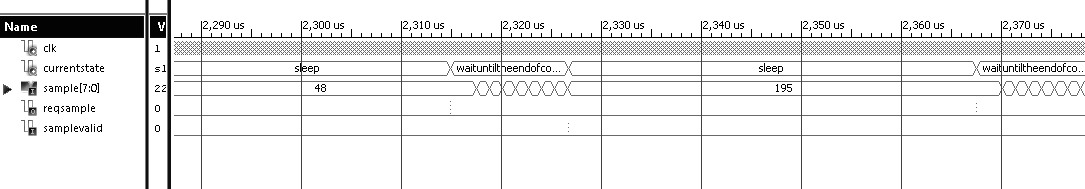
\includegraphics[width=340pt]{waveform-SAMPLER3}
}
\label{fig:waveform-SAMPLER3}
\end{figure}


\clearpage
\begin{figure}[h]
\centering
\setlength\fboxsep{0pt}
\setlength\fboxrule{0.5pt}
\fbox{
	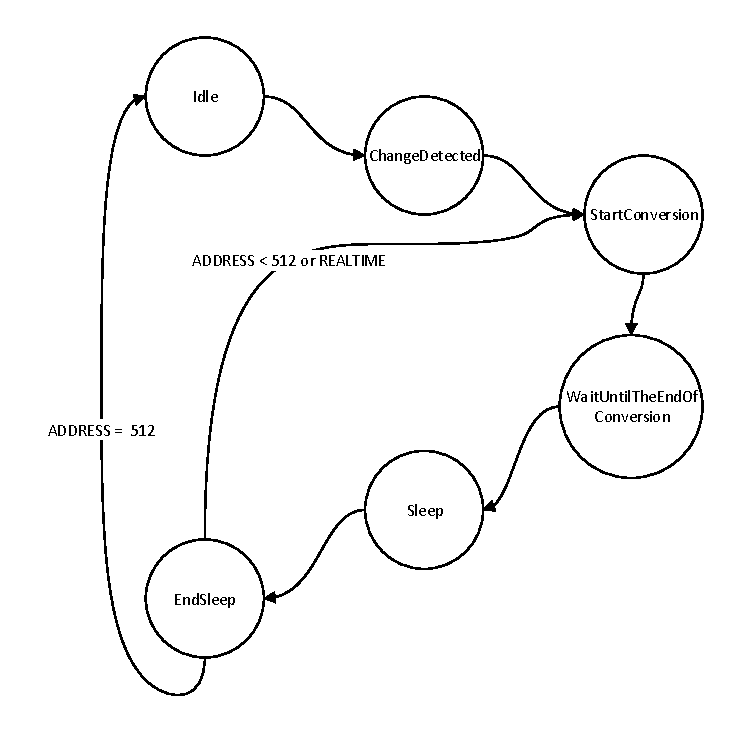
\includegraphics[width=340pt]{SAMPLER-automata}
}
\caption{Diagrama de stare a automatului SAMPLER}
\label{fig:SAMPLER-automata}
\end{figure}



\paragraph{}
Starea \textbf{ChangeDetected} reprezinta starea de initializare a registrului de baleiaj cu adresa 0. Se intra in aceasta stare din \textbf{Idle} cand se detecteaza o schimbare a datelor de pe magistrala \textbf{FREQ}. In starea \textbf{StartConversion} bitul \textbf{REQ\_SAMPLE} devine 1 logic, astfel se semnaleaza o cerere de conversie spre modulul de comunicare (COMM). Se asteapta in starea \textbf{WaitUntilTheEndOfConversion} pana cand bitul \textbf{SAMPLE\_VALID} devine 1 logic iar apoi se intra in starea \textbf{Sleep} in care se incrementeaza un registru la fiecare tact pana la valoarea semnalului \textbf{FREQ}. Cand se atinge aceasta valoare se intra in starea \textbf{EndSleep} de unde se poate continua baleierea adreselor sau inghetarea automatului in starea \textbf{Idle}. Modul de functionare "Timp Real" presupune tranzitia in starea \textbf{StartConversion} iar modul "Captura" tranzitia in starea \textbf{Idle}.


\clearpage

\paragraph{}
Protocolul de comunicare este implementat pe placuta CEREBOT2 folosind intreruperile externe. Cand se detecteaza o tranzitie de tip front crescator al bitului START\_BIT se va genera o intrerupere in care se cere o conversie AD. Valoarea unui registru (de stare) va fi setata pe Waiting. Cand conversia AD este terminata se va genera o alta intrerupere unde se salveaza valoarea convertita intr-un registru. Dupa fiecare intrerupere REQ\_BIT  se va trimite spre iesire valoarea convertita, se va face 1 logic BIT\_VALID iar apoi  registrul se deplasa cu un bit. Daca conversia nu este gata cand vine prima cerere REQ\_BIT vom astepta pana cand va fi gata intr-o stare de Wait (while(1)). BIT\_VALID va deveni 0 de fiecare data cand se executa bucla principala a programului.




\paragraph{}
Pentru testarea in simulator noi am folosit un bloc care genereaza esantioane pseudo- aleatoare cu bistabile si porti xor. Aceasta componenta respecta interfata de comunicare COMM si este o masina de stare.


\begin{figure}[h]
\centering
\setlength\fboxsep{0pt}
\setlength\fboxrule{0.5pt}
\fbox{
	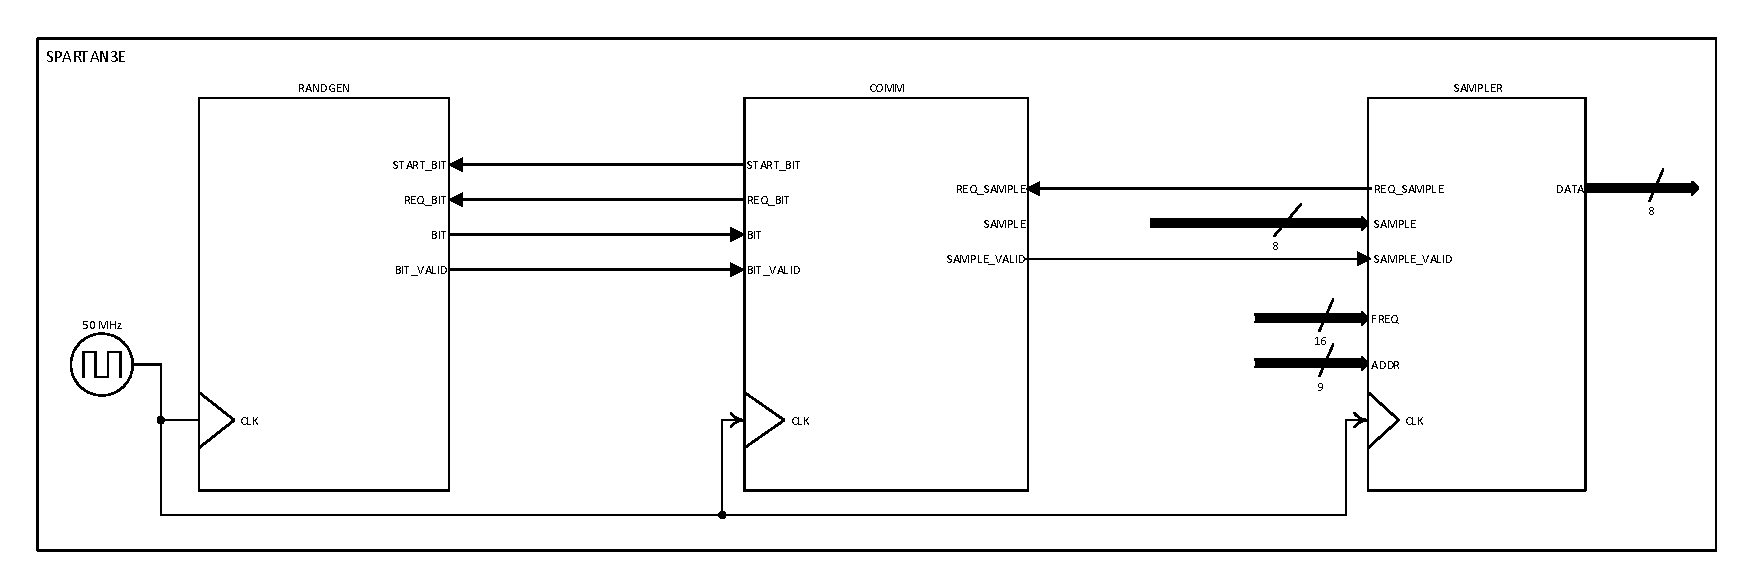
\includegraphics[width=340pt]{oscupdate-rand}
}
\caption{Schema blocului de esantionare cu generator de valori aleatoare pentru testarea in simulator}
\label{fig:oscupdate-rand}
\end{figure}
\subsection{Logica de iesire}
\paragraph{}
Aceasta sectiune a documentului este dedicata implementarii blocului de afisare din Figura \ref{fig:bloc_afisare}.

\paragraph{}
Dupa cum s-a vazut la capitolul de fundamente teoretice, un controller VGA trebuie sa furnizeze cinci semnale: trei pentru culoarea curenta, si 2 pentru sincronizarea fascicolului de electroni. Din fericire, placuta \emph{Basys2} pune la dispozitie 10 semnale pe care le converteste la un port VGA dupa cum urmeaza:

\begin{figure}[h]
\centering
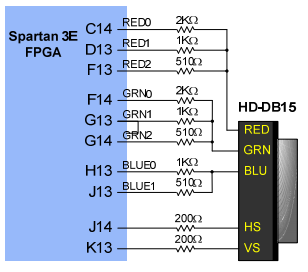
\includegraphics[width=180pt]{basys2_vga}
\caption{Basys2 VGA Port}
\label{fig:vga_pinout}
\end{figure}

Observam ca Basys2 ne pune la dispozitie trei semnale digitale pentru canalul culorii \emph{Rosu}, trei pentru \emph{Verde} si doar 2 pentru \emph{Albastru}. Impreuna formeaza un bus de 8 biti. Culoarea albastra primeste o rezolutie mai mica deoarece ochiul uman este mai sensibil la verde si rosu. Basys2 converteste aceste valori digitale la un semnal analogic pentru fiecare canal. Semnalele pentru sincronizarea orizontala si verticala sunt legate fara logica suplimentara.

\paragraph{}
Deoarece clock-ul placutei Basys2 este de {\tt50Mhz}, putem aproxima o frecventa de {\tt25.157Mhz} impartind la doi frecventa placutei. O frecventa de {\tt25Mhz} este suficienta pentru ca majoritatea monitoarelor sa se recunoasca rezolutia.

\begin{lstlisting}[frame=L]
    if rising_edge(clk) then
        if clk25MHz = '1' then
            -- logica la 25Mhz
        end if;
        clk25MHz <= not clk25MHz;
    end if;
\end{lstlisting}

\paragraph{}
Din pacate, oscilatorul placutei Basys2 nu este suficient de stabil pentru a sincroniza monitoarele moderne. Se recomanda folosirea unui oscilator separat, conectat la slotul dedicat al placutei. Autorii proiectului nu au avut acces la un oscilator stabil. Imaginea rezultata folosind oscilatorul nativ sufera de artefacte verticale. Cu toate acestea, forma de unda este vizibila si poate fi recunoscuta de catre utilizator.

\clearpage
\paragraph{}
Componenta de control a logicii de iesire are ca semnal de intrare impulsul de clock, iar ca semnale de iesire pozitia pe X si Y a fascicolului de electroni pe suprafata monitorului, impreuna cu un semnal de control care indica daca fascicolul se afla pe suprafata vizibila sau nu.

\paragraph{}
Folosind doua comparatoare, se determina daca pozitia fascicolului pe verticala ( axa Y ) se afla intre valorile esantioanelor de la adresele X, respectiv X-1. Aceasta metoda presupune ca dimensiunea memoriei de esantionare este egala cu rezolutia verticala a monitorului in pixeli, iar valorile esantioanelor sunt scalate in prealabil pentru a fi mapate direct in spatiul monitorului.

Pentru a face comparatia intre pozitia curenta si valoarea a doua esantioane intr-un singur impuls de clock ( respectiv doua, luand in considerare faptul ca fascicolul de electroni petrece doua semnale de clock deasupra unui pixel, frecventa clock-ului intern al  controllerului VGA fiind jumatate din frecventa clock-ului placutei ), se memoreaza valoarea esantionului de pe pozitia anterioara intr-un bistabil D. Daca pozitia curenta a fascicolului se afla intre valorile esantioanelor, culoarea trimisa la portul VGA este cea alba, adica \emph{"11111111"}. In caz contrar, sau daca fascicolul se afla in afara zonei vizibile, culoarea trimisa este cea neagra, respectiv \emph{"00000000"}. Acest lucru se face folosind un multiplexor legat la o logica combinationala ce foloseste valorile de iesire ale comparatoarelor, si semnalul ce indica daca fascicolul se afla in zona vizuala sau nu.

\begin{figure}[h]
\centering
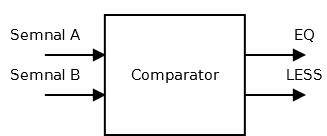
\includegraphics[width=180pt]{comparator}
\caption{Comparator}
\label{fig:comparator}
\end{figure}


Comparatoarele sunt circuite combinationale ce primesc ca semnale de intrare doua valori de comparat, si prezinta la iesire doua semnale digitale numite \emph{EQ} si \emph{LESS}, active pe '1' logic, ce au ca semnificatie:

\begin{center}
    \begin{tabular}{| l | l | l |}
    \hline
    EQ & LESS & Interpretare \\ \hline
	1 & * & Semnalele sunt egale  \\ \hline
    0 & 0 & Semnalul A este mai mic decat B  \\ \hline
    0 & 1 & Semnalul A este mai mare decat B \\ \hline 
    \end{tabular}
\end{center}

\clearpage
\begin{figure}[h]
\centering
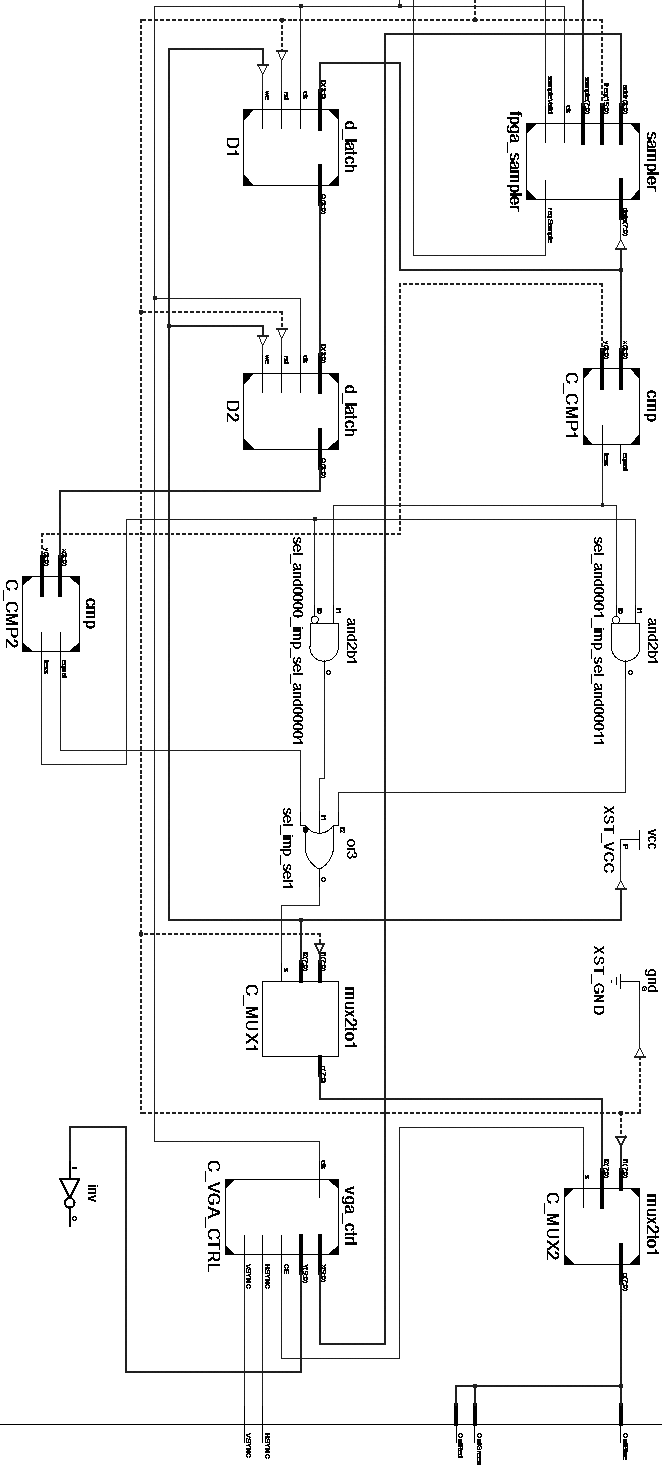
\includegraphics[width=320pt]{vga_rtl}
\caption{Schema pentru logica de iesire}
\label{fig:vga_rtl}
\end{figure}
\clearpage

\section{Rezultate experimentale}
\clearpage

\section{Concluzii}
\paragraph{}
In primul rand acest proiect este mai mult didactic si nu poate inlocui solutii care sunt mai eficiente din punct de vedere calitate/pret. Contributia noastra a fost determinarea componentelor unui osciloscop digital si implementarea acestuia pe o placuta FPGA in limbajul VHDL. Automatele de stare au fost folosite excesiv pentru controlul componentelor, astfel demonstrandu-se puterea lor in a rezolva probleme de timp real.
\paragraph{}
Design-ul ofera un anumit grad de flexibilitate, osciloscopul avand posibilitatea de a fi conectat la orice monitor VGA si la orice sistem de achizitie atat timp cat se respecta protocolul de comunicare (COMM).
\paragraph{}
Pentru entuziasti, sistemul poate fi folosit pentru verificarea unor semnale analogice cu conditia ca acestea sa aiba tensiunea suportata de ADC-ul placutei CEREBOT 2. Sistemul poate fi extins adaugand module care sa afiseze date statistice sau auxiliare pe monitorul VGA, cum ar fi o legenda de timp, sau frecventa si amplitudinea undei detectate.

\begin{thebibliography}{99}

\bibitem{lamport94}
  Leslie Lamport,
  \emph{\LaTeX: A Document Preparation System}.
  Addison Wesley, Massachusetts,
  2nd Edition,
  1994.

\bibitem{wikiosc}
 Analog and Digital Oscilloscope\\
\url{ http://en.wikipedia.org/wiki/Oscilloscope}

\bibitem{oscqa}
 Practical questions and answers about oscilloscope use\\
\url{ http://forum.allaboutcircuits.com/showthread.php?t=2645 }

\bibitem{basys2}
 Basys 2 Reference Manual\\
\url{ http://www.digilentinc.com/Data/Products/BASYS2/Basys2\_rm.pdf }

\bibitem{vga}
 VGA controller and specification\\
\url{ http://www.eng.utah.edu/~cs3710/labs/VGA.pdf }

\bibitem{vga2}
 Hardware Design with VHDL : VGA Example\\
\url{ http://www.ece.unm.edu/~jimp/vhdl_fpgas/slides/VGA.pdf }

\bibitem{vga3}
 VGA Timings\\
\url{ http://hamsterworks.co.nz/mediawiki/index.php/VGA_timings }


\bibitem{cerebot2}
 Cerebot II Reference Manual\\
\url{ http://www.digilentinc.com/Data/Products/CEREBOT-II/Cerebot\_II\_rm\_RevB.pdf }
\end{thebibliography}

\end{document}
